\subsection{User Interfaces}
\label{subsect:User Interfaces}
	The following mockups are a representation of the look of the app in its first release.
	\subsubsection{Login}
	\begin{figure}[H]
	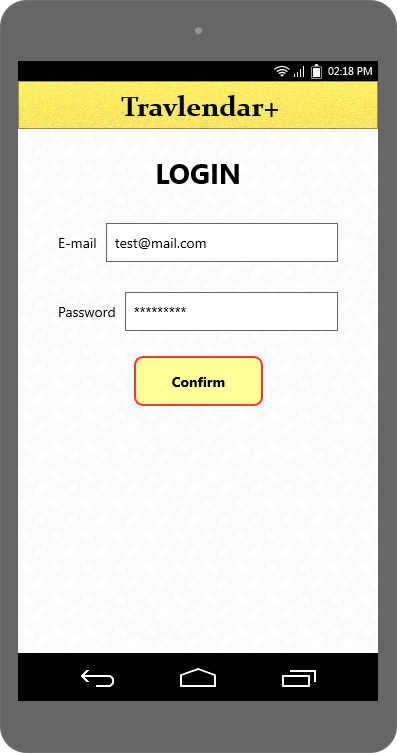
\includegraphics[scale=0.35]{mockup/app/03-Login}
	\vspace{2.5cm}
	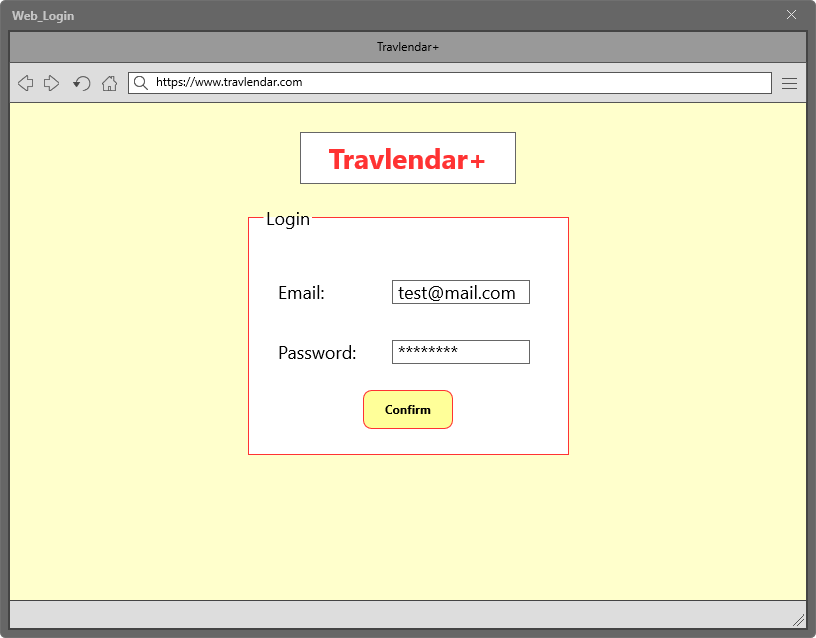
\includegraphics[scale=0.35]{mockup/web/01-Web_Login}
	\centering 
	\end{figure}
	
	\subsubsection{Calendar and Map views}
	\begin{figure}[H]
	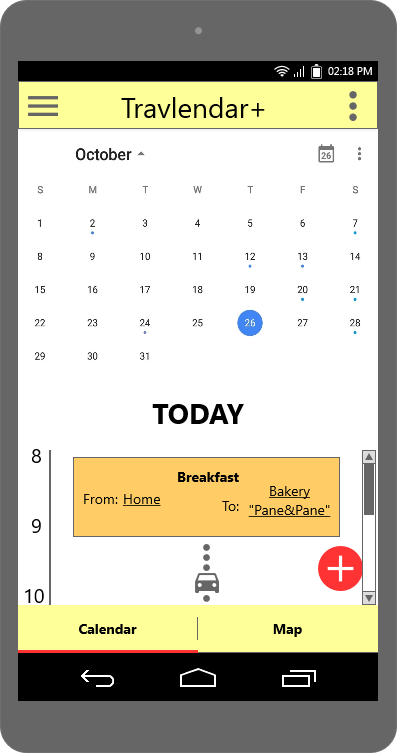
\includegraphics[scale=0.35]{mockup/app/04-Calendar}
	\hspace{2.5cm}
	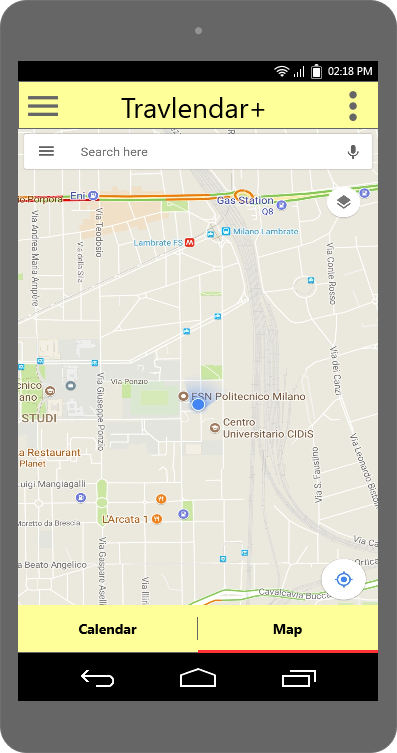
\includegraphics[scale=0.35]{mockup/app/06-Map}
	\centering 
	\end{figure}
	
	\subsubsection{Day Viewer and Event Creation}
	\begin{figure}[H]
	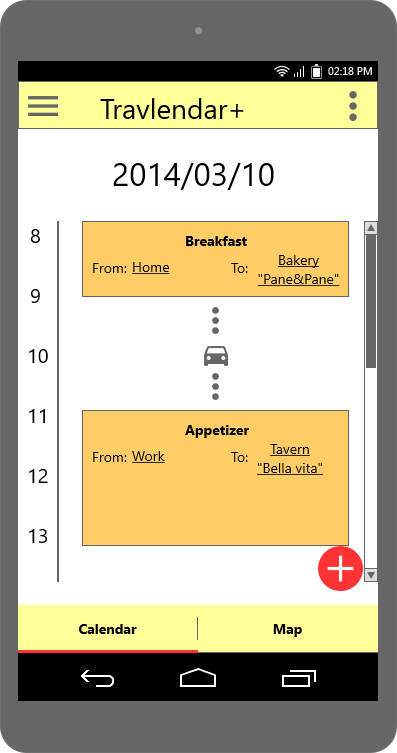
\includegraphics[scale=0.35]{mockup/app/05-Day_Viewer}
	\hspace{2.5cm}
	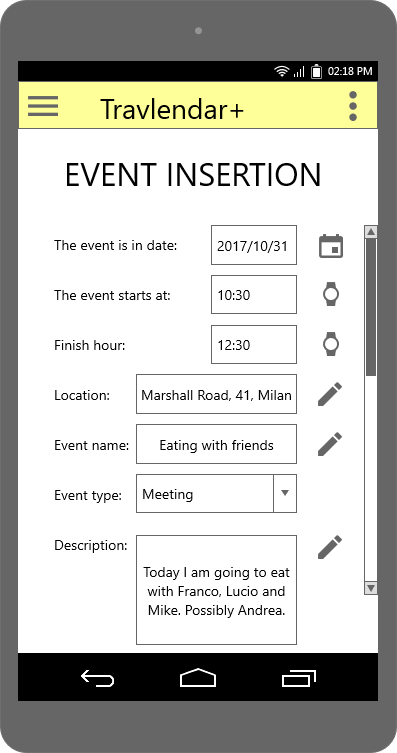
\includegraphics[scale=0.35]{mockup/app/11-Create_Event}
	\centering 
	\end{figure}
	
	\subsubsection{My Tickets and Preferences}
	\begin{figure}[H]
	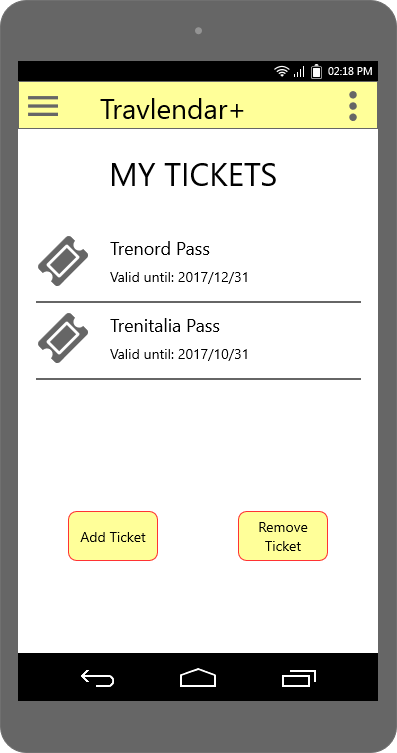
\includegraphics[scale=0.4]{mockup/app/09-My_Tickets}
	\hspace{2.5cm}
	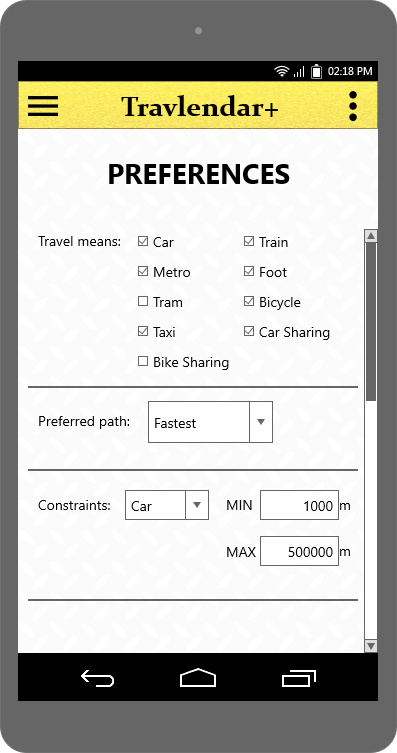
\includegraphics[scale=0.4]{mockup/app/08-Preferences}
	\centering 
	\end{figure}
	
	\subsubsection{WebApp View}
	\begin{figure}[H]
	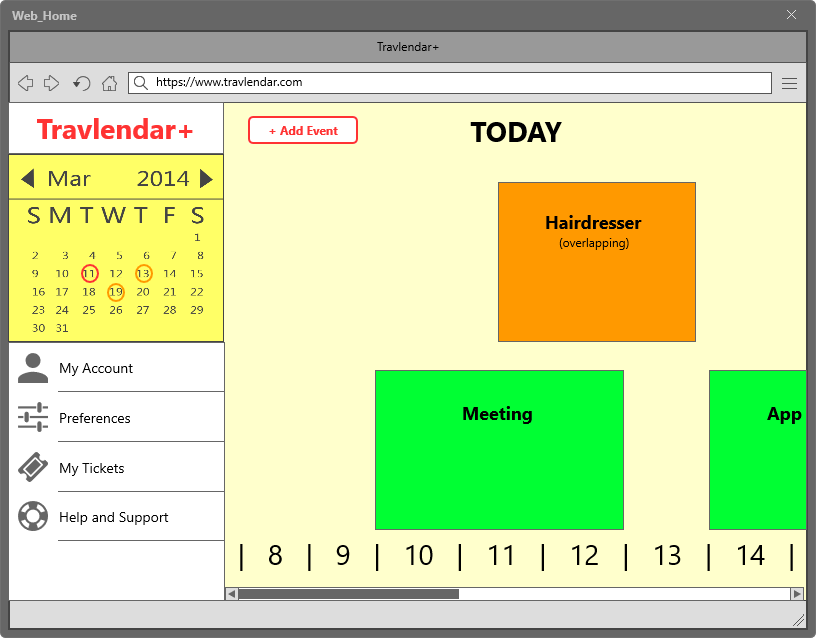
\includegraphics[scale=0.4]{mockup/web/02-Web_Home}
	\centering 
	\end{figure}
\subsection{Hardware Interfaces}
\label{subsect:Hardware Interfaces}
	The mobile app is supported on:
	\begin{itemize}
		\item Android 6.0 and superior;
		\item iOS 8 and superior;
	\end{itemize}
	To utilize the mobile app, the phone must be able to connect to the Internet and have a working GPS sensor to identify its position. \\ \\
	The web app is supported on these browsers:
	\begin{itemize}
		\item Google Chrome;
		\item Mozilla Firefox;
		\item Microsoft Edge;
		\item Safari;
	\end{itemize}
	Other browsers may be utilized to access the web app, but full compatibility is not guaranteed.
\subsection{Software Interfaces}
\label{subsect:Software Interfaces}
	This system implements Google Maps APIs to calculate the optimal travel path to reach a destination. \\
	Interaction with external websites of travel means providers is required in order to allow the user to buy tickets.
\subsection{Communication Interfaces}
\label{subsect:Communication Interfaces}
	During the registration phase, the system will automatically send an email to the email address inserted by the user. This email will contain a recap of the data inserted by the user during the registration, along with a link that needs to be clicked by the user in order to verify that the email is currently valid and active.